% Editable source for the heavy-chain example in dynamic.md.
% From this directory, regenerate with:
% latex -interaction=nonstopmode -halt-on-error dynamic.tex
% dvisvgm --no-fonts --exact --bbox=papersize --output=dynamic.svg dynamic.dvi
\documentclass[tikz,border=5pt]{standalone}
\usepackage{lmodern}
\begin{document}
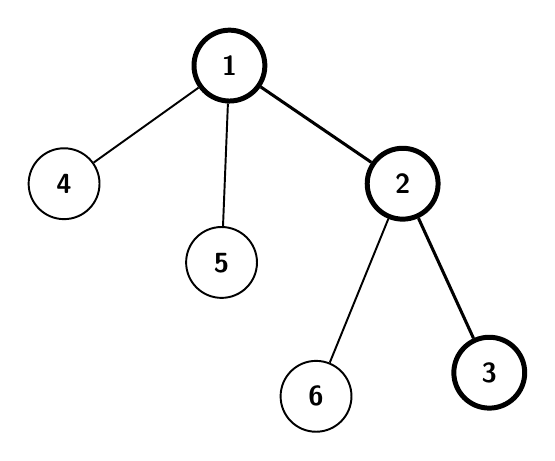
\begin{tikzpicture}[
  vertex/.style={circle,draw,fill=white,minimum size=9mm,inner sep=0pt,
    font=\sffamily\bfseries,line width=0.7pt},
  heavy/.style={vertex,line width=1.8pt},
  line width=0.7pt
]
  % The heavy chain is 1--2--3. Vertices 4, 5 and 6 are light children.
  \node[heavy] (v1) at (0,0) {1};
  \node[heavy] (v2) at (2.2,-1.5) {2};
  \node[heavy] (v3) at (3.3,-3.9) {3};
  \node[vertex] (v4) at (-2.1,-1.5) {4};
  \node[vertex] (v5) at (-0.1,-2.5) {5};
  \node[vertex] (v6) at (1.1,-4.2) {6};
  \draw (v1) -- (v4) (v1) -- (v5) (v2) -- (v6);
  \draw[line width=1.1pt] (v1) -- (v2) -- (v3);
\end{tikzpicture}
\end{document}
